\section{Contadores}

El hecho de que el flip flop presente una entrada de clock que habilite
un cambio de estado a la salida, permite que se puedan implementar
los flip flops para contar una cantidad de ciclos de clocks que han
transcurrido en el tiempo. Este dispositivo que permite construir
la implementación con flip flops es llamado contador, y existen dos
tipos los cuales son: asincrónico y contador sincrónico.
A continuación se presenta una implementación de flip flops tipo ''T''
para el contador asincrónico y para el contador sincrónico:

\begin{figure}[H]
\centering
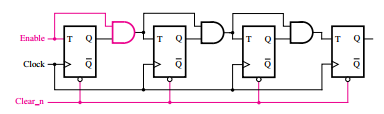
\includegraphics[scale=0.7]{sincCOUNTER.PNG}
\qquad
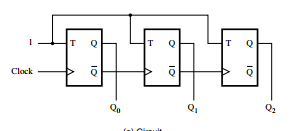
\includegraphics[scale=0.7]{asincCOUNTER.PNG}
\caption{Contador sincrónico y asincrónico}
\end{figure}

Como se puede ver en el diseño del contador sincrónico (imagen de
la izquierda), los flip flops habilitan el cambio de estado al mismo
tiempo (la entrada de clock es la misma para todos, clock sincrónico),
mientras que para el contador asincrónico la entrada de clock de los
flip flops proviene del flip flop anterior. Esto último provoca en
los contadores asincrónicos una dependencia mayor del delay de los
flip flops en su funcionamiento.

\subsection{Implementación}

En esta parte del artículo se propone implementar un contador de 3
bits (uno asincrónico y otro sincrónico) e intentar medir su máxima
velocidad de operación. El diseño a utilizar es el mismo que el presentado
en la imagen anterior (con solo tres flip flops, uno por bit) pero
con flip flops tipo D. Para lograr esto se propuso el siguiente diseño
para lograr un flip flop tipo T a partir de uno tipo D y así poder
realizar los contadores:

\begin{figure}[H]
\centering
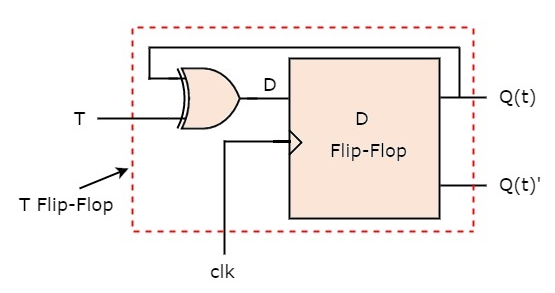
\includegraphics[scale=0.4]{TflipflopWithD.PNG}
\caption{Flip Flop tipo T a partir del tipo D.}
\end{figure}


\subsection{Máxima Velocidad de Operación}

Para lograr estimar la máxima velocidad de operación, se aumentó la
frecuencia del clock hasta que esta fue lo suficientemente elevada
para que los flip flops no pudieran seguir el conteo correctamente.
Lo que ocurrió fue que el contador asincrónico cesó de operar adecuadamente
a una frecuencia de clock de $21MHz$ mientras que el contador sincrónico
lo hizo a una frecuencia de clock de $45MHz$.

Esto tiene sentido, ya que según la datasheet de los flip flops utilizados
el tiempo de propagación es del orden de los $20ns$. Esto quiere
decir que a una frecuencia $f=\frac{1}{20ns}=50MHz$ es esperable
que el contador no actualice la cuenta a tiempo. Esto es para el flip
flop sincrónico, pero para el asincrónico el tiempo de progragación
se multiplica por la cantidad de bits del contador, o lo que es lo
mismo, por la cantidad de flip flops. Para el caso del contador de
tres bits, la frecuencia de operación se reduce a un tercio de la
que se tenía para el sincrónico.

Vale aclarar que lo estimado teóricamente con los parámetros de la
hoja de datos y lo medido no se ajusta perfectamente a la realidad, pero esto es
esperable debido a las dificultades de medir con el osciloscopio en
altas frecuencias de trabajo y además porque no solo existen flip
flops en el circuito, si no que se han utilizado otras compuertas
como las AND y las XOR que no han sido incorporadas en el análisis. De
todas maneras, se puede notar que el contador sincrónico permite aumentar
más la frecuencia de trabajo (respecto al asincrónico)
sin que se afecte el funcionamiento.